\documentclass{standalone}
\usepackage{tikz}
\usetikzlibrary{patterns, positioning}
\usepackage[sfdefault]{ClearSans} %% option 'sfdefault' activates Clear Sans as the default text font
\usepackage[T1]{fontenc}

\begin{document}
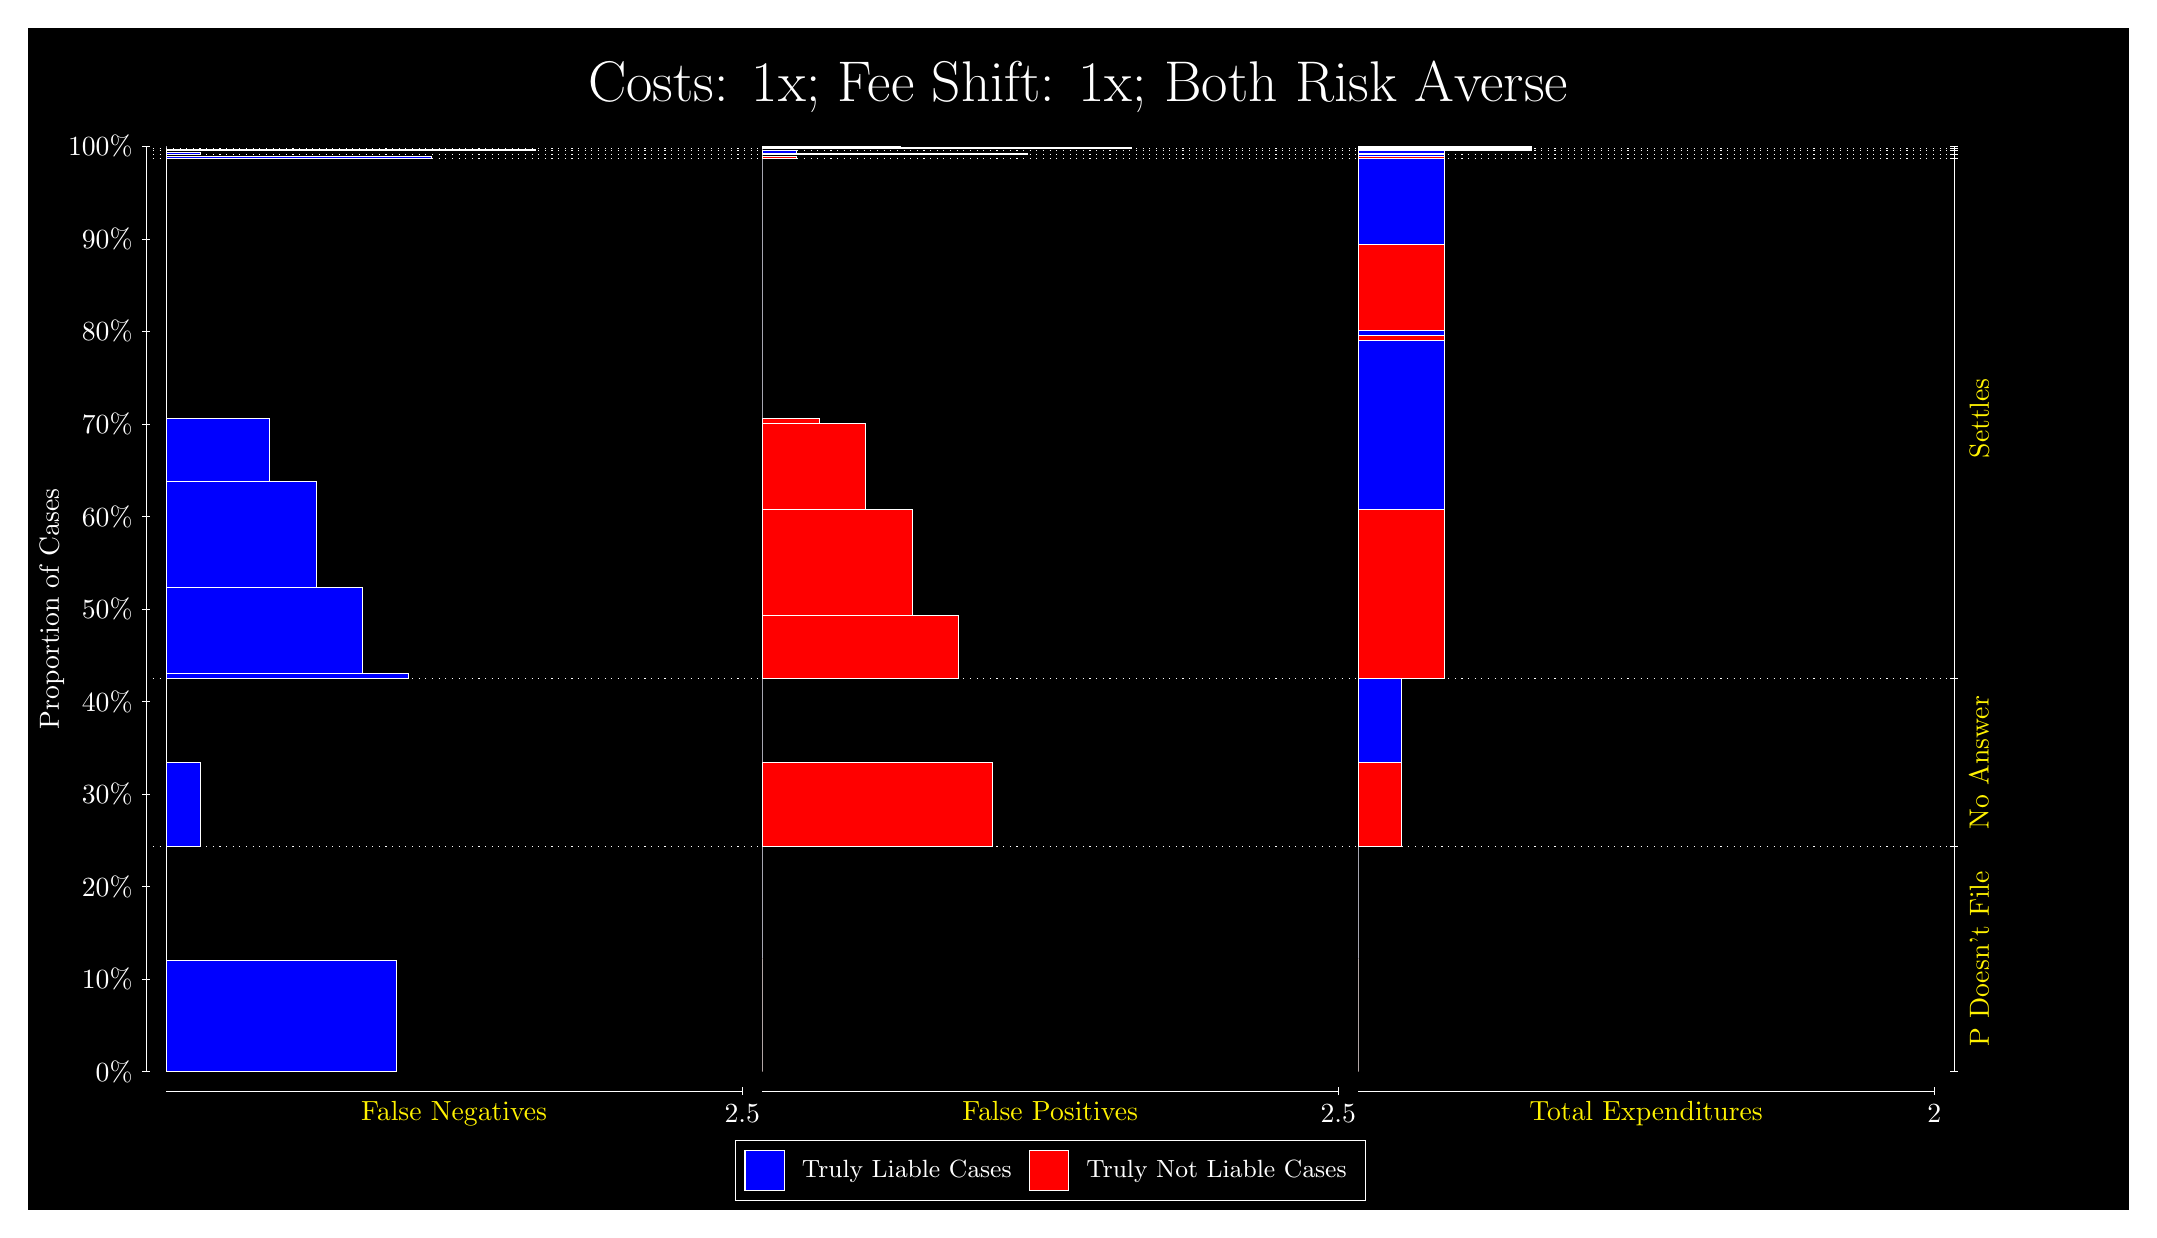
\begin{tikzpicture}
\draw[fill=black] (0,0) rectangle (26.667,15);
\draw[text=white] (0,13.5) rectangle (26.667,15) node[midway] {\huge Costs: 1x; Fee Shift: 1x; Both Risk Averse};
\draw[white, very thin] (1.5,1.75) -- (1.5,13.5);
\node[rotate=90, text=white, anchor=center] at (0.3, 7.625) {Proportion of Cases};
\draw[white, very thin] (1.45,1.75) -- (1.55,1.75);
\node[text=white, anchor=east] at (1.45, 1.75) {0\%};
\draw[white, very thin] (1.45,2.925) -- (1.55,2.925);
\node[text=white, anchor=east] at (1.45, 2.925) {10\%};
\draw[white, very thin] (1.45,4.1) -- (1.55,4.1);
\node[text=white, anchor=east] at (1.45, 4.1) {20\%};
\draw[white, very thin] (1.45,5.275) -- (1.55,5.275);
\node[text=white, anchor=east] at (1.45, 5.275) {30\%};
\draw[white, very thin] (1.45,6.45) -- (1.55,6.45);
\node[text=white, anchor=east] at (1.45, 6.45) {40\%};
\draw[white, very thin] (1.45,7.625) -- (1.55,7.625);
\node[text=white, anchor=east] at (1.45, 7.625) {50\%};
\draw[white, very thin] (1.45,8.8) -- (1.55,8.8);
\node[text=white, anchor=east] at (1.45, 8.8) {60\%};
\draw[white, very thin] (1.45,9.975) -- (1.55,9.975);
\node[text=white, anchor=east] at (1.45, 9.975) {70\%};
\draw[white, very thin] (1.45,11.15) -- (1.55,11.15);
\node[text=white, anchor=east] at (1.45, 11.15) {80\%};
\draw[white, very thin] (1.45,12.325) -- (1.55,12.325);
\node[text=white, anchor=east] at (1.45, 12.325) {90\%};
\draw[white, very thin] (1.45,13.5) -- (1.55,13.5);
\node[text=white, anchor=east] at (1.45, 13.5) {100\%};

\draw[white, very thin] (24.457,1.75) -- (24.457,13.5);
\draw[white, very thin] (24.407,1.75) -- (24.507,1.75);
\node[anchor=west] at (24.407, 1.75) {};
\draw[white, very thin] (24.407,4.6066) -- (24.507,4.6066);
\node[anchor=west] at (24.407, 4.6066) {};
\draw[white, very thin] (24.407,6.7429) -- (24.507,6.7429);
\node[anchor=west] at (24.407, 6.7429) {};
\draw[white, very thin] (24.407,13.349) -- (24.507,13.349);
\node[anchor=west] at (24.407, 13.349) {};
\draw[white, very thin] (24.407,13.393) -- (24.507,13.393);
\node[anchor=west] at (24.407, 13.393) {};
\draw[white, very thin] (24.407,13.447) -- (24.507,13.447);
\node[anchor=west] at (24.407, 13.447) {};
\draw[white, very thin] (24.407,13.473) -- (24.507,13.473);
\node[anchor=west] at (24.407, 13.473) {};
\draw[white, very thin] (24.407,13.5) -- (24.507,13.5);
\node[anchor=west] at (24.407, 13.5) {};

\draw[white, very thin, fill=blue] (1.75,1.75) rectangle (4.6775,3.1687);
\draw[white, very thin, fill=red] (1.75,3.1687) rectangle (1.75,4.6066);
\draw[white, very thin, fill=blue] (1.75,4.6066) rectangle (2.1891,5.6747);
\draw[white, very thin, fill=red] (1.75,5.6747) rectangle (1.75,6.7429);
\draw[white, very thin, fill=blue] (1.75,6.7429) rectangle (4.8239,6.8026);
\draw[white, very thin, fill=blue] (1.75,6.8026) rectangle (4.2384,7.8995);
\draw[white, very thin, fill=blue] (1.75,7.8995) rectangle (3.6529,9.2471);
\draw[white, very thin, fill=blue] (1.75,9.2471) rectangle (3.0674,10.048);
\draw[white, very thin, fill=red] (1.75,10.048) rectangle (1.75,13.349);
\draw[white, very thin, fill=blue] (1.75,13.349) rectangle (5.1167,13.371);
\draw[white, very thin, fill=red] (1.75,13.371) rectangle (1.75,13.393);
\draw[white, very thin, fill=blue] (1.75,13.393) rectangle (2.1891,13.425);
\draw[white, very thin, fill=red] (1.75,13.425) rectangle (1.75,13.447);
\draw[white, very thin, fill=blue] (1.75,13.447) rectangle (6.4341,13.46);
\draw[white, very thin, fill=red] (1.75,13.46) rectangle (1.75,13.473);
\draw[white, very thin, fill=red] (1.75,13.473) rectangle (1.75,13.485);
\draw[white, very thin, fill=blue] (1.75,13.485) rectangle (1.75,13.5);
\draw[white, very thin, fill=red] (9.3189,1.75) rectangle (9.3189,3.1879);
\draw[white, very thin, fill=blue] (9.3189,3.1879) rectangle (9.3189,4.6066);
\draw[white, very thin, fill=red] (9.3189,4.6066) rectangle (12.246,5.6748);
\draw[white, very thin, fill=blue] (9.3189,5.6748) rectangle (9.3189,6.7429);
\draw[white, very thin, fill=red] (9.3189,6.7429) rectangle (11.807,7.5441);
\draw[white, very thin, fill=red] (9.3189,7.5441) rectangle (11.222,8.888);
\draw[white, very thin, fill=red] (9.3189,8.888) rectangle (10.636,9.979);
\draw[white, very thin, fill=red] (9.3189,9.979) rectangle (10.051,10.044);
\draw[white, very thin, fill=blue] (9.3189,10.044) rectangle (9.3189,13.349);
\draw[white, very thin, fill=red] (9.3189,13.349) rectangle (9.758,13.371);
\draw[white, very thin, fill=blue] (9.3189,13.371) rectangle (9.3189,13.393);
\draw[white, very thin, fill=red] (9.3189,13.393) rectangle (12.686,13.414);
\draw[white, very thin, fill=blue] (9.3189,13.414) rectangle (9.758,13.447);
\draw[white, very thin, fill=red] (9.3189,13.447) rectangle (9.3189,13.46);
\draw[white, very thin, fill=blue] (9.3189,13.46) rectangle (9.3189,13.473);
\draw[white, very thin, fill=red] (9.3189,13.473) rectangle (14.003,13.485);
\draw[white, very thin, fill=blue] (9.3189,13.485) rectangle (11.075,13.5);
\draw[white, very thin, fill=red] (16.888,1.75) rectangle (16.888,3.1879);
\draw[white, very thin, fill=blue] (16.888,3.1879) rectangle (16.888,4.6066);
\draw[white, very thin, fill=red] (16.888,4.6066) rectangle (17.437,5.6748);
\draw[white, very thin, fill=blue] (16.888,5.6748) rectangle (17.437,6.7429);
\draw[white, very thin, fill=red] (16.888,6.7429) rectangle (17.986,8.888);
\draw[white, very thin, fill=blue] (16.888,8.888) rectangle (17.986,11.037);
\draw[white, very thin, fill=red] (16.888,11.037) rectangle (17.986,11.101);
\draw[white, very thin, fill=blue] (16.888,11.101) rectangle (17.986,11.161);
\draw[white, very thin, fill=red] (16.888,11.161) rectangle (17.986,12.252);
\draw[white, very thin, fill=blue] (16.888,12.252) rectangle (17.986,13.349);
\draw[white, very thin, fill=red] (16.888,13.349) rectangle (17.986,13.371);
\draw[white, very thin, fill=blue] (16.888,13.371) rectangle (17.986,13.393);
\draw[white, very thin, fill=red] (16.888,13.393) rectangle (17.986,13.414);
\draw[white, very thin, fill=blue] (16.888,13.414) rectangle (17.986,13.447);
\draw[white, very thin, fill=red] (16.888,13.447) rectangle (19.083,13.46);
\draw[white, very thin, fill=blue] (16.888,13.46) rectangle (19.083,13.473);
\draw[white, very thin, fill=red] (16.888,13.473) rectangle (19.083,13.485);
\draw[white, very thin, fill=blue] (16.888,13.485) rectangle (19.083,13.5);
\draw[white, dotted] (1.5,4.6066) -- (24.457,4.6066);
\draw[white, dotted] (1.5,6.7429) -- (24.457,6.7429);
\draw[white, dotted] (1.5,13.349) -- (24.457,13.349);
\draw[white, dotted] (1.5,13.393) -- (24.457,13.393);
\draw[white, dotted] (1.5,13.447) -- (24.457,13.447);
\draw[white, dotted] (1.5,13.473) -- (24.457,13.473);
\draw[white, very thin] (1.75,1.5) -- (9.0689,1.5);
\node[text=yellow, anchor=north] at (5.4094, 1.5) {False Negatives};
\draw[white, very thin] (9.0689,1.45) -- (9.0689,1.55);
\node[text=white, anchor=north] at (9.0689, 1.45) {2.5};

\draw[white, very thin] (9.3189,1.5) -- (16.638,1.5);
\node[text=yellow, anchor=north] at (12.978, 1.5) {False Positives};
\draw[white, very thin] (16.638,1.45) -- (16.638,1.55);
\node[text=white, anchor=north] at (16.638, 1.45) {2.5};

\draw[white, very thin] (16.888,1.5) -- (24.207,1.5);
\node[text=yellow, anchor=north] at (20.547, 1.5) {Total Expenditures};
\draw[white, very thin] (24.207,1.45) -- (24.207,1.55);
\node[text=white, anchor=north] at (24.207, 1.45) {2};

\node[text=yellow, centered, rotate=90] at (24.777, 3.1783) {P Doesn't File};
\node[text=yellow, centered, rotate=90] at (24.777, 5.6747) {No Answer};
\node[text=yellow, centered, rotate=90] at (24.777, 10.046) {Settles};





\draw (12.978300999999998,1.5) node[draw=none] (baseCoordinate) {};
\begin{scope}[align=center]
        \matrix[scale=0.5, draw=white, below=0.5cm of baseCoordinate, nodes={draw}, column sep=0.1cm]{
            \node[rectangle, draw, minimum width=0.5cm, minimum height=0.5cm, fill=blue] {}; &
            \node[draw=none, font=\small, text=white] (B) {Truly Liable Cases}; &
            \node[rectangle, draw, minimum width=0.5cm, minimum height=0.5cm, fill=red] {}; &
            \node[draw=none, font=\small, text=white] (B) {Truly Not Liable Cases}; \\
            };
\end{scope}

\end{tikzpicture}
\end{document}